% XeLaTeX document
\documentclass[12pt,a4paper]{article}

% Редактируем: конфигурация, личные настройки: имя, название предмета и пр. для титульной страницы и метаданных документа здесь
\newcommand{\university}{Национальный исследовательский Университет ИТМО}
\newcommand{\mfaculty}{Мегафакультет информационных и трансляционных технологий}
\newcommand{\faculty}{Факультет инфокоммуникационных технологий}
\newcommand{\city}{Санкт-Петербург}
\newcommand{\num}{№6}
\newcommand{\docname}{Типовой расчет }
\newcommand{\subject}{Математический анализ}
\newcommand{\tutorname}{Ю.В. Танченко}
\newcommand{\studentname}{В.М. Касьяненко}
\newcommand{\group}{K3121}

% Не редактируем: используемые пакеты
% настройка кодировки, шрифтов и русского языка
\usepackage{fontspec}
\usepackage{polyglossia}

% рабочие ссылки в документе
\usepackage{hyperref}

% графика
\usepackage{graphicx}
\usepackage{tikz}

% поворот страницы
\usepackage{pdflscape}

% качественные листинги кода
\usepackage{minted}
\usepackage{listings}
\usepackage{lstfiracode}

% отключение копирования номеров строк из листинга, работает не во всех просмотрщиках (в Adobe Reader работает)
\usepackage{accsupp}
\newcommand\emptyaccsupp[1]{\BeginAccSupp{ActualText={}}#1\EndAccSupp{}}
\let\theHFancyVerbLine\theFancyVerbLine
\def\theFancyVerbLine{\rmfamily\tiny\emptyaccsupp{\arabic{FancyVerbLine}}}

% библиография
\bibliographystyle{templates/gost-numeric.bbx}
\usepackage{csquotes}
\usepackage[parentracker=true,backend=biber,hyperref=true,bibencoding=utf8,style=numeric-comp,language=auto,autolang=other,citestyle=gost-numeric,defernumbers=true,bibstyle=gost-numeric,sorting=ntvy]{biblatex}

% установка полей
\usepackage{geometry}

% нумерация картинок по секциям
\usepackage{chngcntr}

% дополнительные команды для таблиц
\usepackage{booktabs}

% для заголовков
\usepackage{caption}
\usepackage{titlesec}
\usepackage[dotinlabels]{titletoc}

% разное для математики
\usepackage{amsmath, amsfonts, amssymb, amsthm, mathtools}

% водяной знак на документе, см. main.tex
\usepackage[printwatermark]{xwatermark}

% Не редактируем: параметры используемых пакетов и не только
% настройки polyglossia
\setdefaultlanguage{russian}
\setotherlanguage{english}

% локализация
\addto\captionsrussian{
	\renewcommand{\figurename}{Рисунок}%
	\renewcommand{\partname}{Глава}
	\renewcommand{\contentsname}{\centerline{Содержание}}
	\renewcommand{\listingscaption}{Листинг}
}

% основной шрифт документа
\setmainfont{CMU Serif}
\newfontfamily\cyrillicfont{CMU Serif}[Script=Cyrillic]

% перечень использованных источников
\addbibresource{refs.bib}

% настройка полей
\geometry{top=2cm}
\geometry{bottom=2cm}
\geometry{left=2cm}
\geometry{right=2cm}
\geometry{bindingoffset=0cm}

% настройка ссылок и метаданных документа
\hypersetup{unicode=true,colorlinks=true,linkcolor=red,citecolor=green,filecolor=magenta,urlcolor=cyan,
	pdftitle={\docname},
	pdfauthor={\studentname},
	pdfsubject={\subject},
	pdfcreator={\studentname},
	pdfproducer={Overleaf},
	pdfkeywords={\subject}
}

% настройка подсветки кода и окружения для листингов
\usemintedstyle{colorful}
\newenvironment{code}{\captionsetup{type=listing}}{}

% шрифт для листингов с лигатурами
\setmonofont{FiraCode-Regular.otf}[
	SizeFeatures={Size=10},
	Path = templates/,
	Contextuals=Alternate
]

% оформления подписи рисунка
\captionsetup[figure]{labelsep = period}

% подпись таблицы
\DeclareCaptionFormat{hfillstart}{\hfill#1#2#3\par}
\captionsetup[table]{format=hfillstart,labelsep=newline,justification=centering,skip=-10pt,textfont=bf}

% путь к каталогу с рисунками
\graphicspath{{fig/}}

% Внесение titlepage в учёт счётчика страниц
\makeatletter
\renewenvironment{titlepage} {
	\thispagestyle{empty}
}
\makeatother

\counterwithin{figure}{section}
\counterwithin{table}{section}

\titlelabel{\thetitle.\quad}

% для удобного конспектирования математики
\mathtoolsset{showonlyrefs=true}
\theoremstyle{plain}
\newtheorem{theorem}{Теорема}[section]
\newtheorem{proposition}[theorem]{Утверждение}
\theoremstyle{definition}
\newtheorem{corollary}{Следствие}[theorem]
\newtheorem{problem}{Задача}[section]
\theoremstyle{remark}
\newtheorem*{nonum}{Решение}

% настоящее матожидание
\newcommand{\MExpect}{\mathsf{M}}

% объявили оператор!
\DeclareMathOperator{\sgn}{\mathop{sgn}}

% перенос знаков в формулах (по Львовскому)
\newcommand*{\hm}[1]{#1\nobreak\discretionary{} {\hbox{$\mathsurround=0pt #1$}}{}}


% водяной знак для обозначения статуса документа
%\newwatermark[allpages,color=red!5,angle=45,scale=3,xpos=0,ypos=0]{DRAFT}
\begin{document}
% Не редактируем: Титульная страница (формируется автоматически из заданной конфигурации)
\begin{titlepage}	% начало титульной страницы

	\begin{center}		% выравнивание по центру

		\large \university \\
		\large \mfaculty \\
		\large \faculty \\[6cm]
		% название института, затем отступ 6см

		\huge \subject \\[0.5cm] % название работы, затем отступ 0,5см
		\large \docname  \num \\[5.1cm]
		 %\large Разработка методов обучения с подкреплением\\[5cm]

	\end{center}


	\begin{flushright} % выравнивание по правому краю
		\begin{minipage}{0.25\textwidth} % врезка в половину ширины текста
			\begin{flushleft} % выровнять её содержимое по левому краю

				\large\textbf{Работу выполнил:}\\
				\large \studentname \\
				\large {Группа:} \group \\

				\large \textbf{Преподаватель:}\\
				\large \tutorname

			\end{flushleft}
		\end{minipage}
	\end{flushright}

	\vfill % заполнить всё доступное ниже пространство

	\begin{center}
		\large \city \\
		\large \the\year % вывести дату
	\end{center} % закончить выравнивание по центру

\end{titlepage} % конец титульной страницы

\vfill % заполнить всё доступное ниже пространство


% Не редактируем: Страница содержания (формируется автоматически из section, subsection и пр., указанных в content.tex)
% Содержание
\tableofcontents
\newpage



% Редактируем: всё остальное: вступление, др. этапы, заключение, приложение
\section*{Введение}
В данной работе будет проведено полное исследование заданной функции, взятой из типового расчета по математике \cite{tip}: 
\begin{equation}
    \centering
    \label{eq:eq1}
    y = \frac{x^2-3}{x-2}.
\end{equation}
 Исследование функции будет проводиться по следующей схеме:
\begin{itemize}
    \item нахождение области значения функции;
    \item проверка на периодичность;
    \item исследование функции с помощью первой производной;
    \item исследование функции с помощью второй производной;
    \item проверка на наличие вертикальных, горизонтальных и наклонных асимптот графика функции;
    \item нахождение точек пересечения графика с координатными осями.
\end{itemize}
\addcontentsline{toc}{section}{Введение}
\newpage
\section{Исследование функции}
\subsection{Область определения функции}
Областью определения функции $\eqref{eq:eq1}$ является вся числовая ось, кроме точки $x = 2$.
\subsection{Проверка на периодичность}
Функция не является периодической. Проверим четность (нечетность):
\[f(-x) = \frac{(-x)^2-3}{-x-2} ;\ f(-x) = \frac{x^2-3}{-x-2} ;\ f(-x) \neq \frac{x^2-3}{x-2} ;\ f(-x) \neq -f(x).\]
Значит, функция не является ни чётной, ни нечётной. График функции не
имеет симметрии ни относительно оси ординат, ни относительно центра
системы координат.
\subsection{Исследование функции с помощью первой производной}
Найдём первую производную функции $\eqref{eq:eq1}$:
\[y' = \left(\frac{x^2-3}{x-2}\right)' = \frac{(x^2-3)'(x-2)-(x^2-3)(x-2)'}{(x-2)^2}  = \frac{x^2-4x+3}{(x-2)^2} = \frac{(x-1)(x-3)}{(x-2)^2}.\]
Тогда $y' = 0$ при $x_1 = 1, x_2 = 3$.
Проверим знаки производной и определим промежутки монотонности функции (рисунок \ref{pic:prom}). Таким образом, функция $\eqref{eq:eq1}$ возрастает при $x \in (-\infty;1) \cup (3; +\infty)$ и убывает при $x \in (1;2) \cup (2;3)$. Далее, так как при переходе через стационарную точку $x = 1$ производная меняет знак с плюса на минус, то $x=1$ точка максимума $(y_{max} = y(1) = 2)$. Аналогично, при переходе через стационарную точку
$x = 3$ производная меняет знак с минуса на плюс, поэтому $x = 3$ точка минимума $(y_{min} = y(3) = 6)$
\begin{figure}[H]
	\begin{center}
		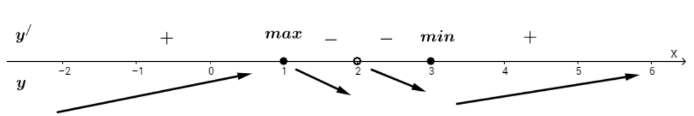
\includegraphics[scale=1]{prom}
		\caption{Промежутки монотонности функции $\eqref{eq:eq1}$}
		\label{pic:prom}
	\end{center}
\end{figure}
\subsection{Исследование функции с помощью второй производной}
Найдём вторую производную функции $\eqref{eq:eq1}$:
\[y'' = \left(\frac{x^2-3}{x-2}\right)'' = \left(\frac{x^2-4x+3}{(x-2)^2}\right)' = \frac{(2x-4)(x-2)^2 - (x^2-4x+3)2(x-2)}{(x-2)^4} = \frac{2}{(x-2)^3}.\]
Проверим знаки второй производной функции и определим промежутки выпуклости (вогнутости) функции (рисунок \ref{pic:vogn}).
\begin{figure}[H]
	\begin{center}
		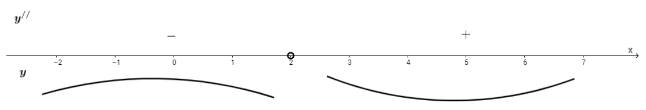
\includegraphics[scale=1.1]{vogn}
		\caption{Промежутки выпуклости (вогнутости) функции $\eqref{eq:eq1}$}
		\label{pic:vogn}
	\end{center}
\end{figure}
Таким образом, функция $\eqref{eq:eq1}$ выпукла вверх при $x \in (-\infty; 2)$ и выпукла вниз (вогнута) при $x \in (2; +\infty)$. Так как точка $x = 2$ не принадлежит области определения функции, она не является и точкой перегиба функции.
\subsection{Проверка на наличие асимптот}
Так как функция $\eqref{eq:eq1}$ не является непрерывной в точке $x = 2$, проверим в этой точке наличие вертикальной асимптоты:
Найдём $\lim\limits_{x\to 2-0} \frac{x^2-3}{x-2} = \frac{1}{-0} = -\infty, \lim\limits_{x\to 2+0} \frac{x^2-3}{x-2} = \frac{1}{+0} = +\infty$, откуда следует, что прямая $x = 2$ является вертикальной асимптотой.
Проверим наличие горизонтальной асимптоты $y = b$: $b = \lim\limits_{x\to \pm \infty} \frac{x^2-3}{x-2} =  \pm \infty \neq const$, откуда следует, что горизонтальной асимптоты нет.
Проверим наличие наклонной асимптоты $y = kx + b$: $k = \lim\limits_{x\to \pm \infty} \frac{f(x)}{x} = \lim\limits_{x\to \pm \infty} \frac{x^2-3}{x(x-2)} = 1,$ $b = \lim\limits_{x\to \pm \infty} f(x) - kx = \lim\limits_{x\to \pm \infty} \left(\frac{x^2-3}{(x-2)}-x\right) = \lim\limits_{x\to \pm \infty} \left(\frac{x^2-3-x(x-2)}{(x-2)}\right) = \lim\limits_{x\to \pm \infty}\left(\frac{2x-3}{x-2}\right) = 2.$
Значит, прямая $y = x + 2$ наклонная асимптота.
\subsection{Нахождение пересечений с осями координат}
Находим точки пересечения функции с координатными осями (таблица \ref{tabular:tab1}): 
\begin{table}[H]
	\caption{Пересечения функции с координатными осями}
	\begin{center}
		\begin{tabular}{|c|c|c|c|}
			\hline
			x & 0 & $\sqrt{3}$ & $-\sqrt{3}$ \\ \hline
			y & 1.5 & 0 & 0 \\ \hline
		\end{tabular}
		\label{tabular:tab1}
	\end{center}
\end{table}
Дополнительные точки: $y(4) = 6,5$; $y(-4) \approx -2,17.$
\section{Построение графика}
\subsection{Построение графика функции по заданию}
График функции представлен на рисунке \ref{pic:gr}:
\begin{figure}[H]
	\begin{center}
		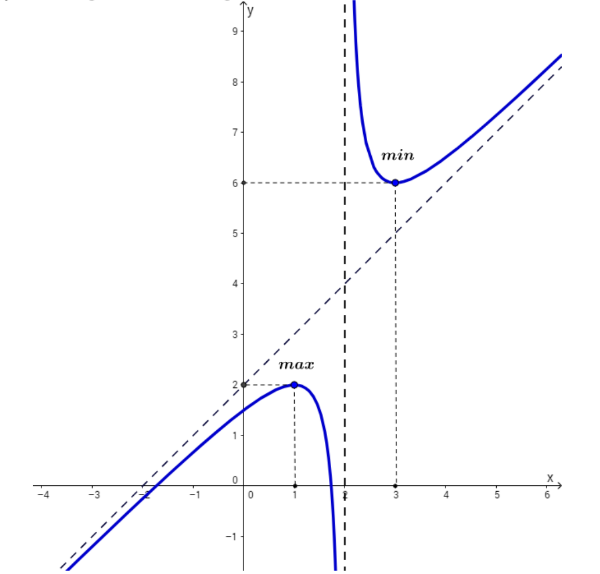
\includegraphics[scale=1]{gr}
		\caption{График функции $\eqref{eq:eq1}$}
		\label{pic:gr} 
	\end{center}
\end{figure}
\subsection{Проверка графика функции}
Проверим построенный график при помощи сайта \cite{desmos}. Введем функцию $\eqref{eq:eq1}$ и получим график, представленный на рисунке \ref{pic:des}:
\begin{figure}[H]
	\begin{center}
		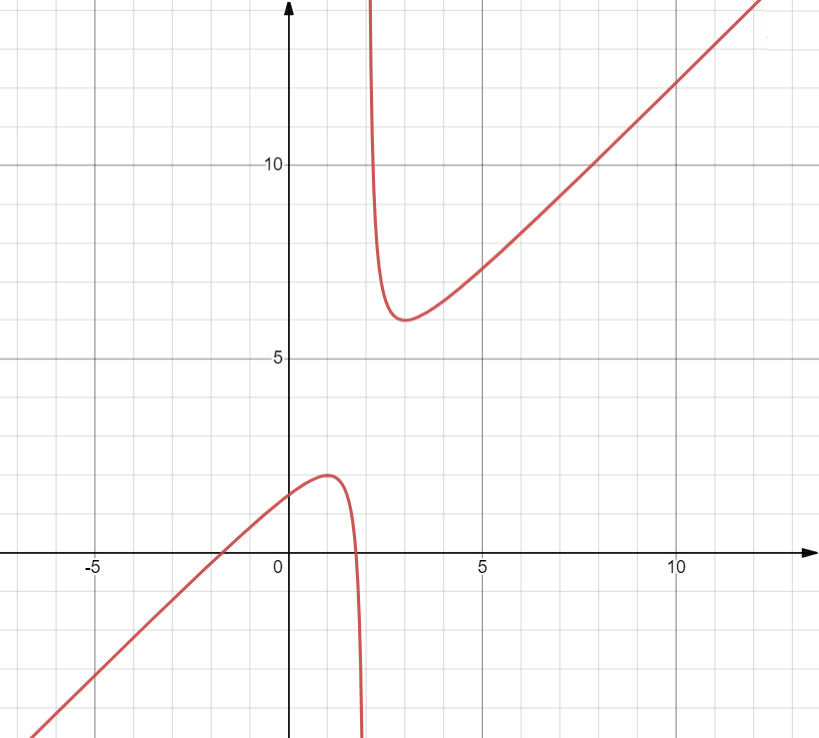
\includegraphics[scale=0.8]{des}
		\caption{График функции $\eqref{eq:eq1}$, построенный сайтом}
		\label{pic:des} 
	\end{center}
\end{figure}
Графики совпадают, следовательно, график функции $\eqref{eq:eq1}$ был построен верно.
\newpage
\section*{Заключение}
В данном типовом расчете была исследована функция $\eqref{eq:eq1}$, а также построен ее график.
\addcontentsline{toc}{section}{Заключение}

% Не редактируем: Страница библиографии (формируется автоматически из книжек, указанных в refs.bib и пометок \cite{имя_источника} в тексте)
\newpage
\printbibliography[title=Список использованных источников]
\addcontentsline{toc}{section}{Список использованных источников}
\end{document}
